\chapter{Aquifer test - Data results (fact sheets)}
\label{chapter:fieldworkresults}
In consultation with Conservation Alliance (CA), a total of five pumping tests are applied in boreholes located at Bingo, Nungo, Nyong Nayili and Janga. By the use of a fifth borehole, location Ziong, the day-to-day PIT system-use is monitored for a week. All tests are applied in November-December 2017, shortly after the transition from wet to dry season. Geohydrological data is gathered by the application of the general pumping test set-up (as described above) at the location Nungo, Nyong Nayili and Janga. The simplified set-up is applied at the location Bingo and Ziong. Outcome of the tests are widespread. Detailed site-specific results are displayed in the fact-sheet figures below (Figures ~\ref{fig:Bingo} -~\ref{fig:Ziong}).

\begin{figure}[h!]
 \centering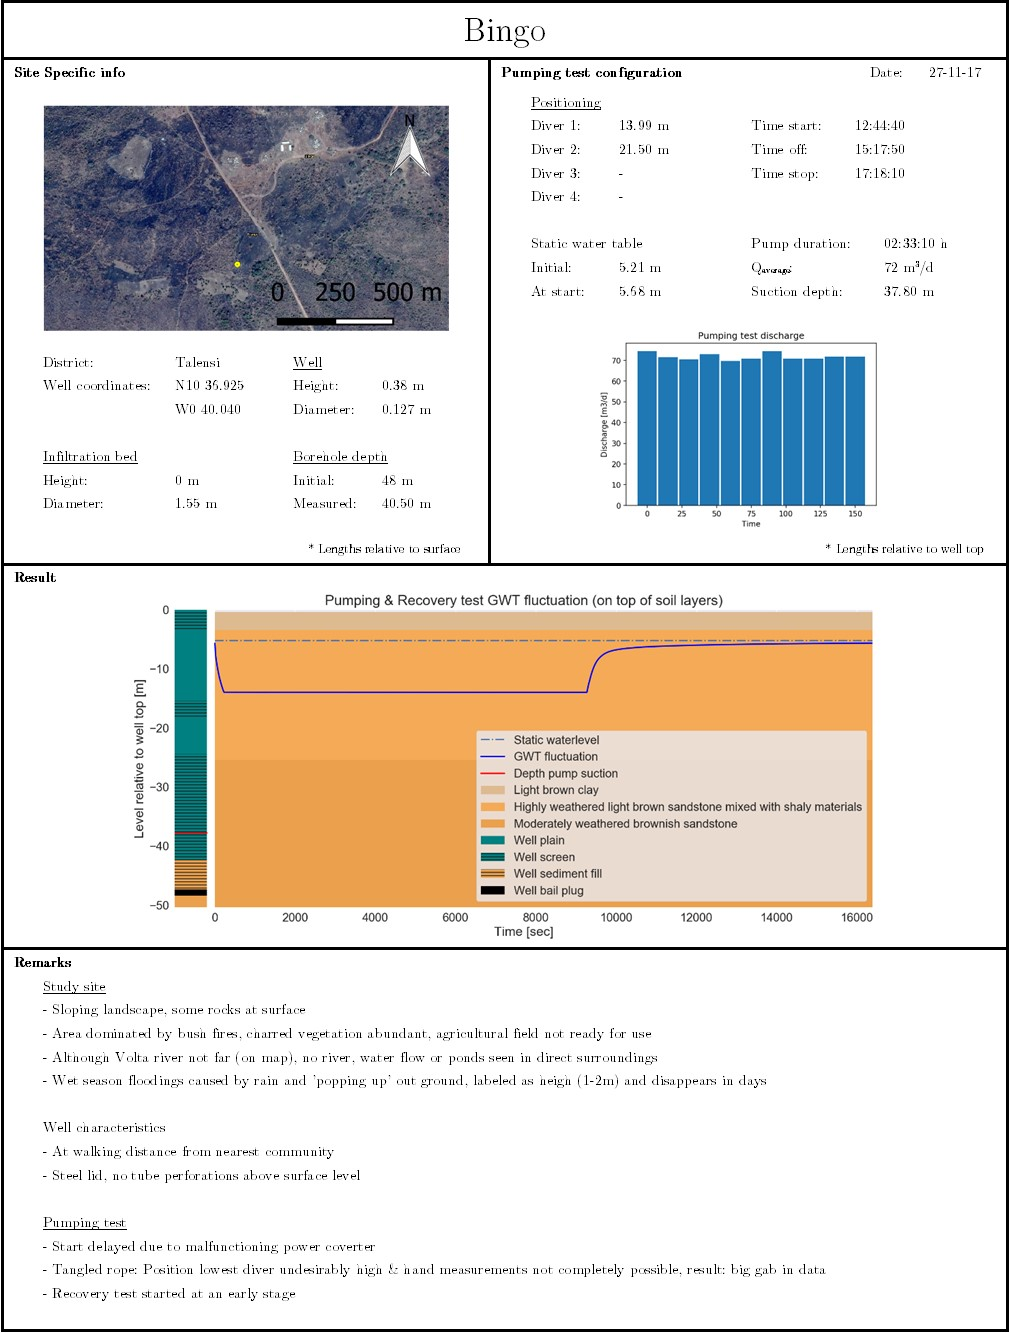
\includegraphics[width=\linewidth]{Bingo.jpg}
 \captionsetup{justification=centering}
 \caption{Fieldwork fact sheet: Bingo}
 \label{fig:Bingo}
\end{figure} 

\begin{figure}[h!]
 \centering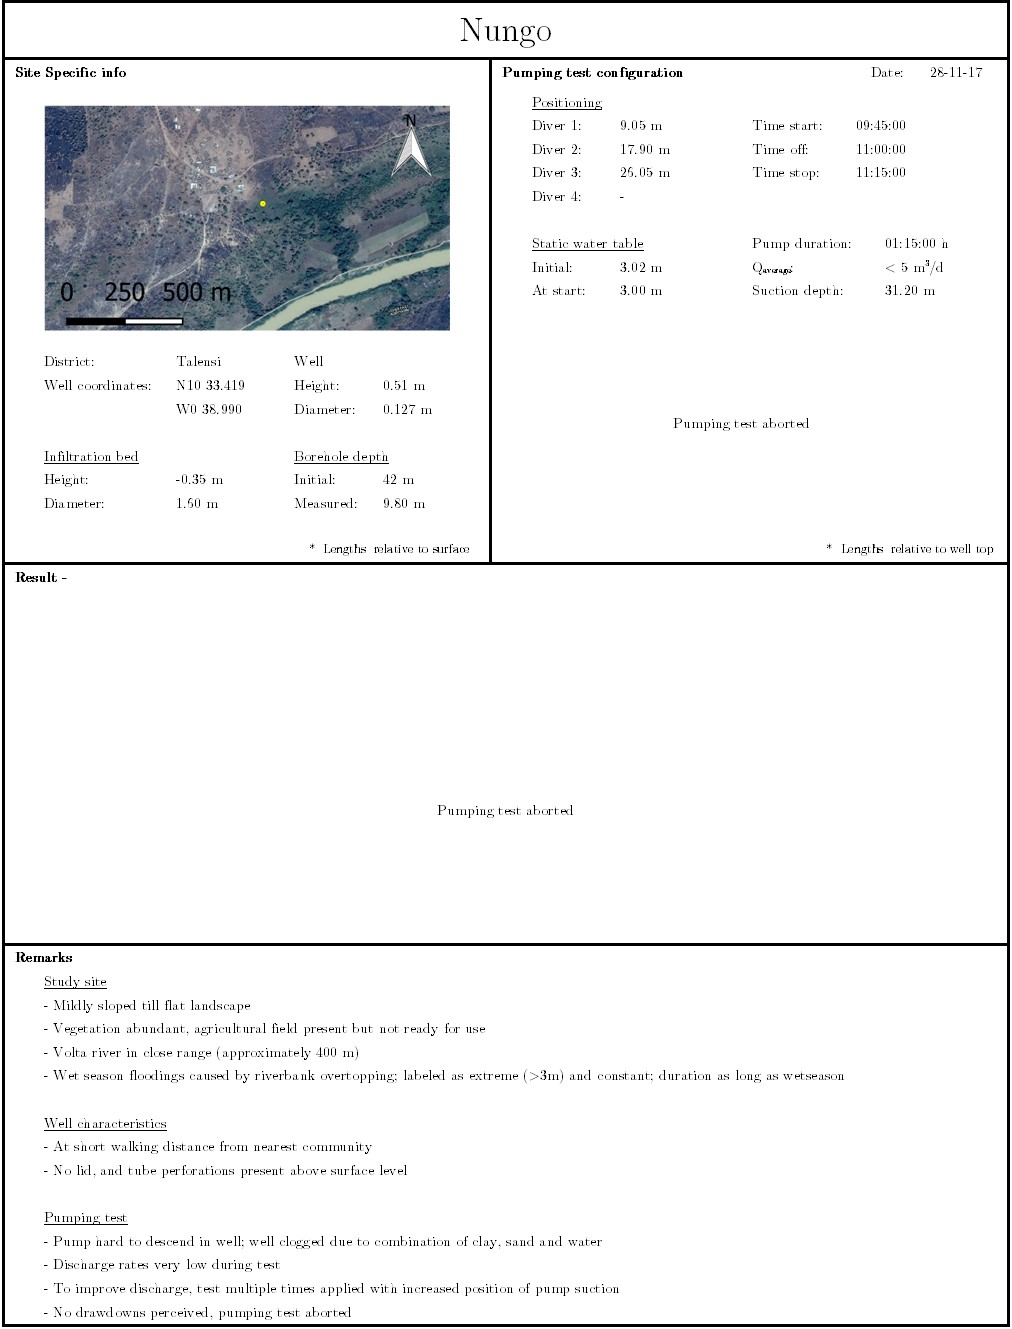
\includegraphics[width=\linewidth]{Nungo.jpg}
 \captionsetup{justification=centering}
 \caption{Fieldwork fact sheet: Nungo}
 \label{fig:Nungo}
\end{figure} 

\begin{figure}[h!]
 \centering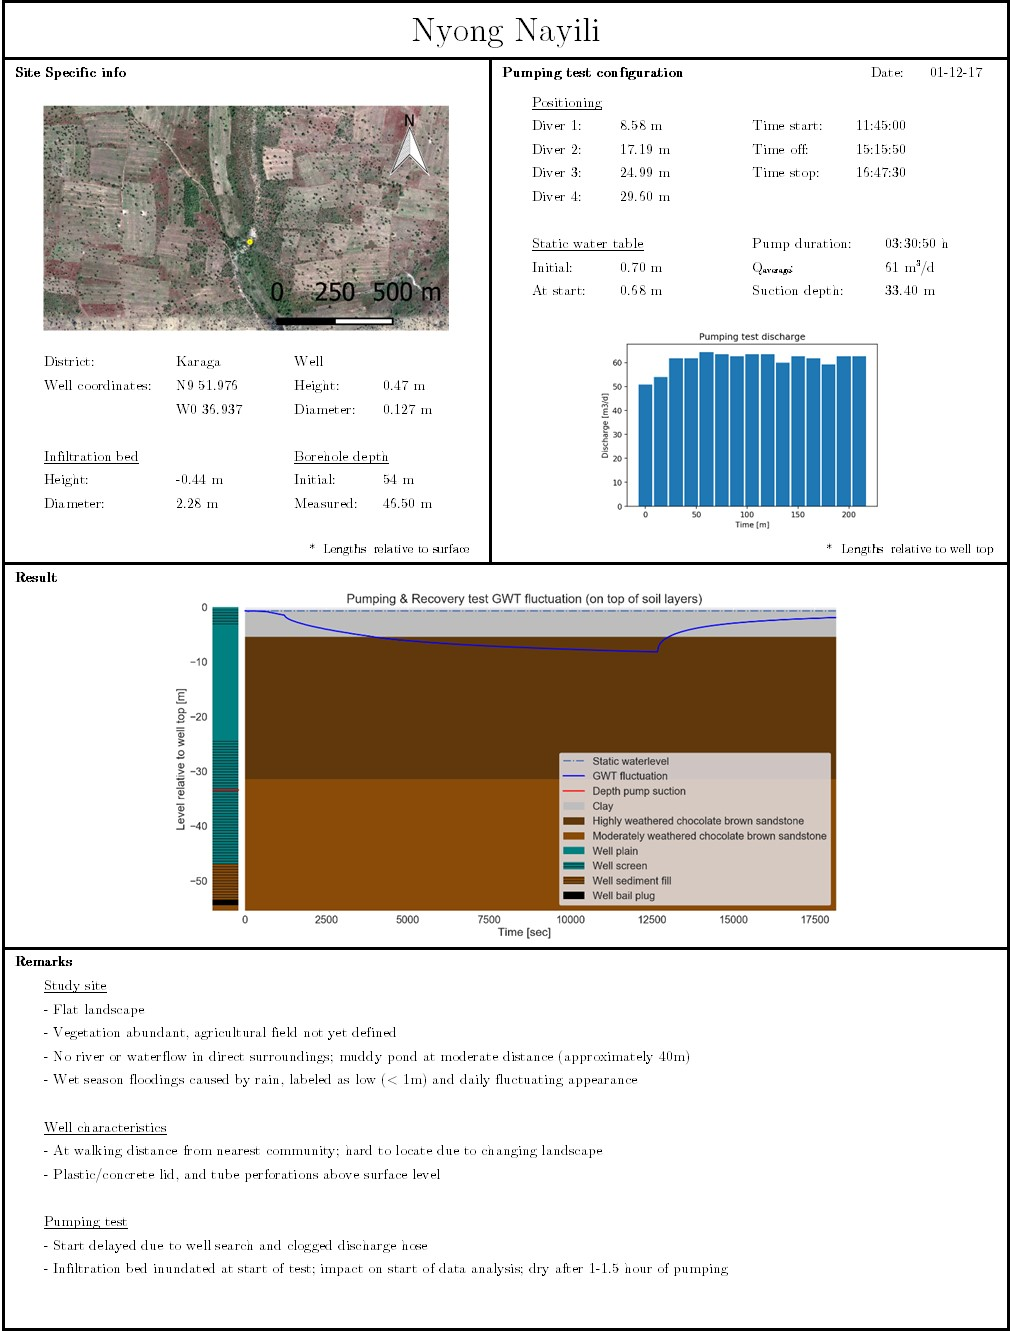
\includegraphics[width=\linewidth]{Nyong_Nayili.jpg}
 \captionsetup{justification=centering}
 \caption{Fieldwork fact sheet: Nyong Nayili}
 \label{fig:Nyong_Nayili}
\end{figure} 

\begin{figure}[h!]
 \centering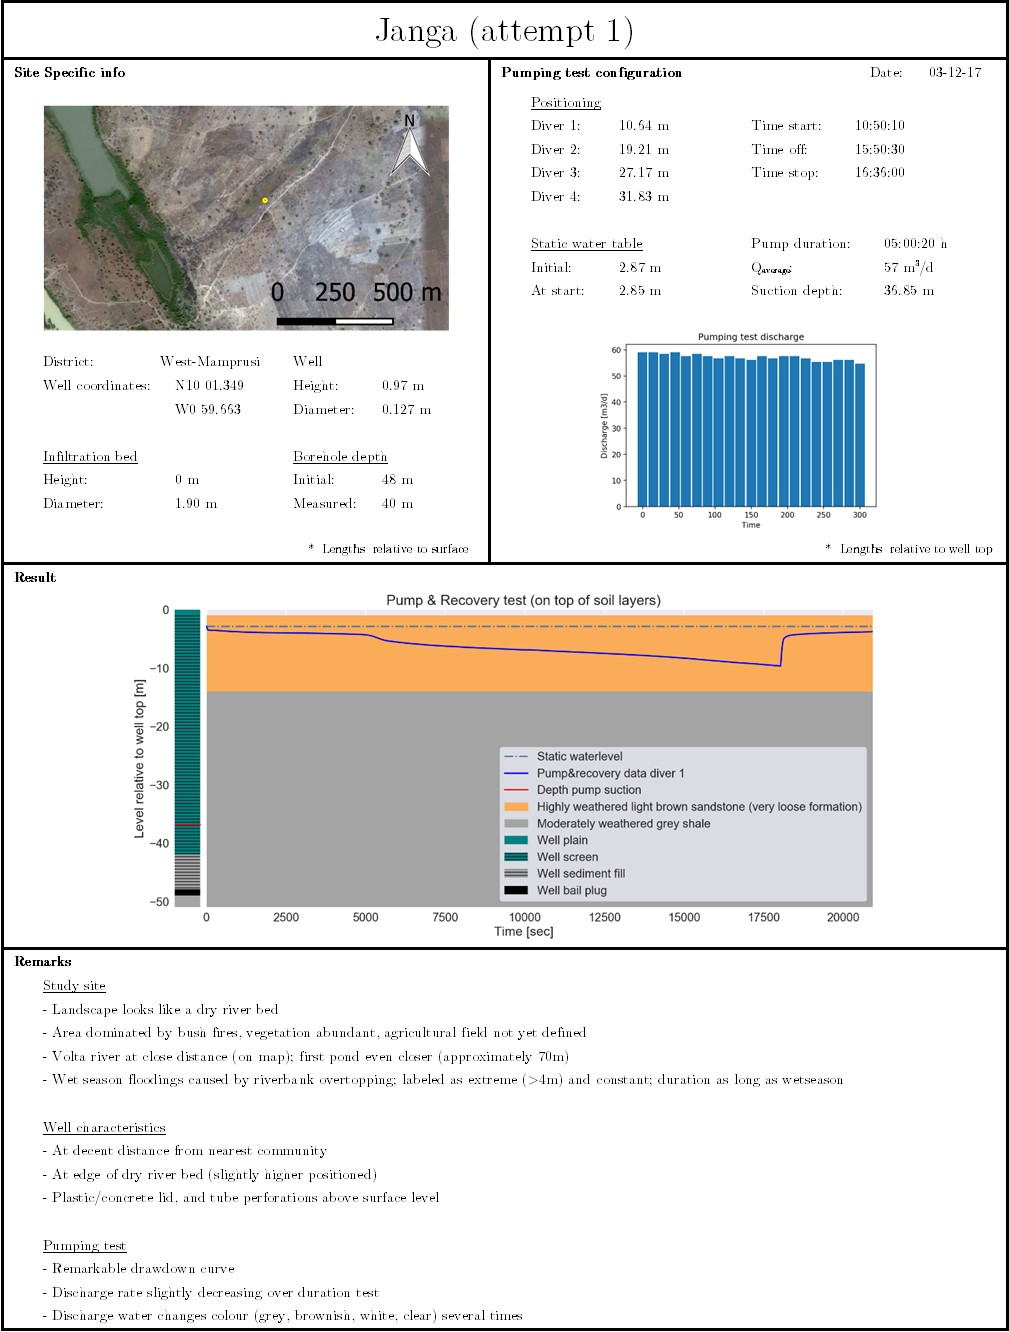
\includegraphics[width=\linewidth]{Janga1.jpg}
 \captionsetup{justification=centering}
 \caption{Fieldwork fact sheet: Janga (attempt 1)}
 \label{fig:Janga1}
\end{figure} 

\begin{figure}[h!]
 \centering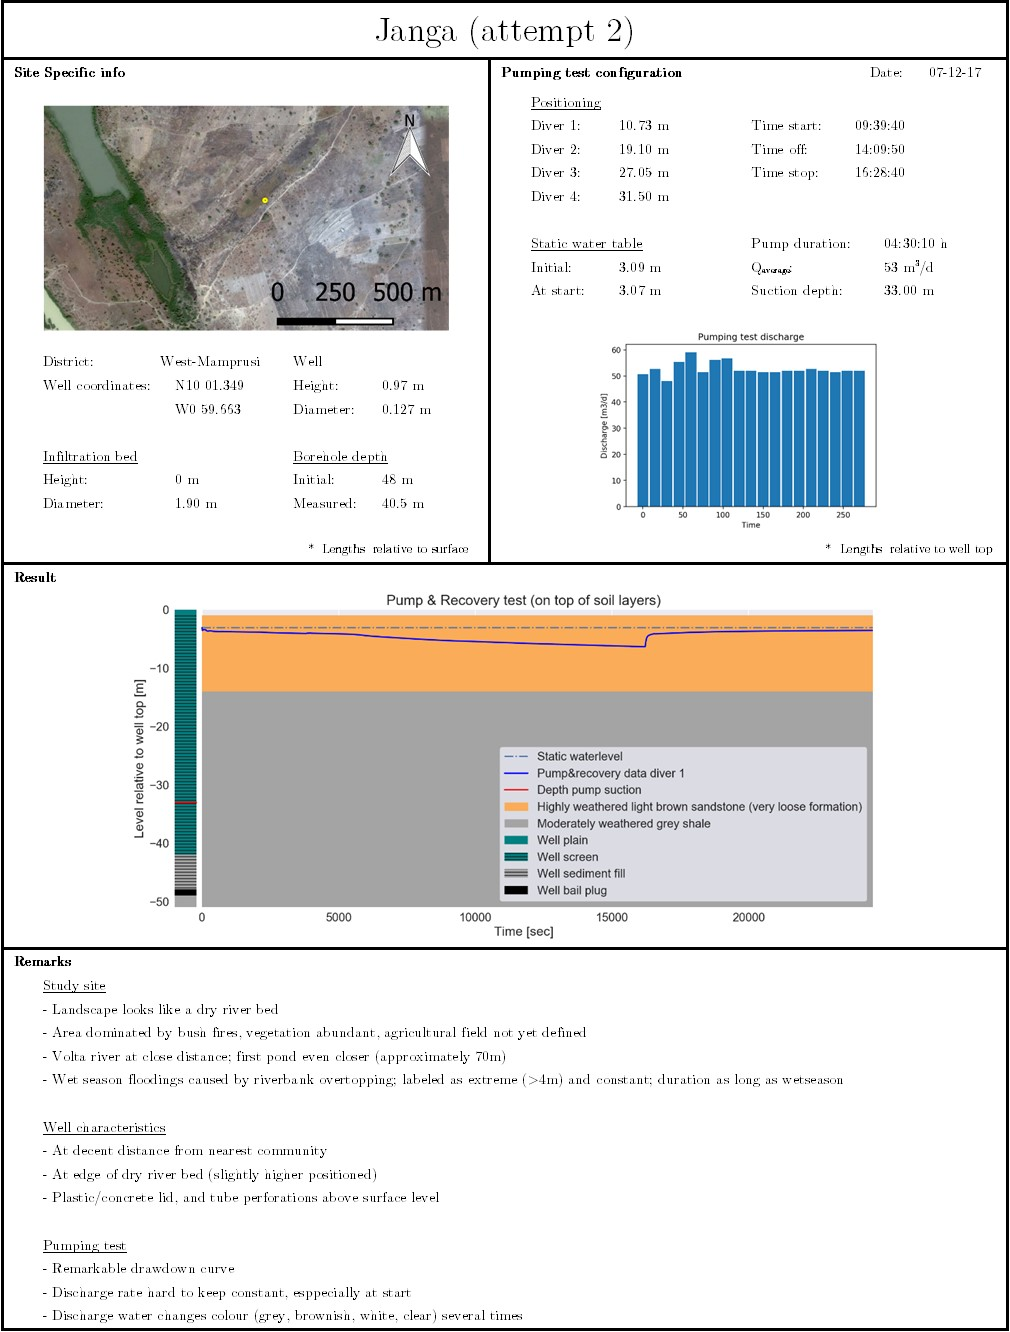
\includegraphics[width=\linewidth]{Janga2.jpg}
 \captionsetup{justification=centering}
 \caption{Fieldwork fact sheet: Jamga (attempt 2)}
 \label{fig:Janga2}
\end{figure} 

\begin{figure}[h!]
 \centering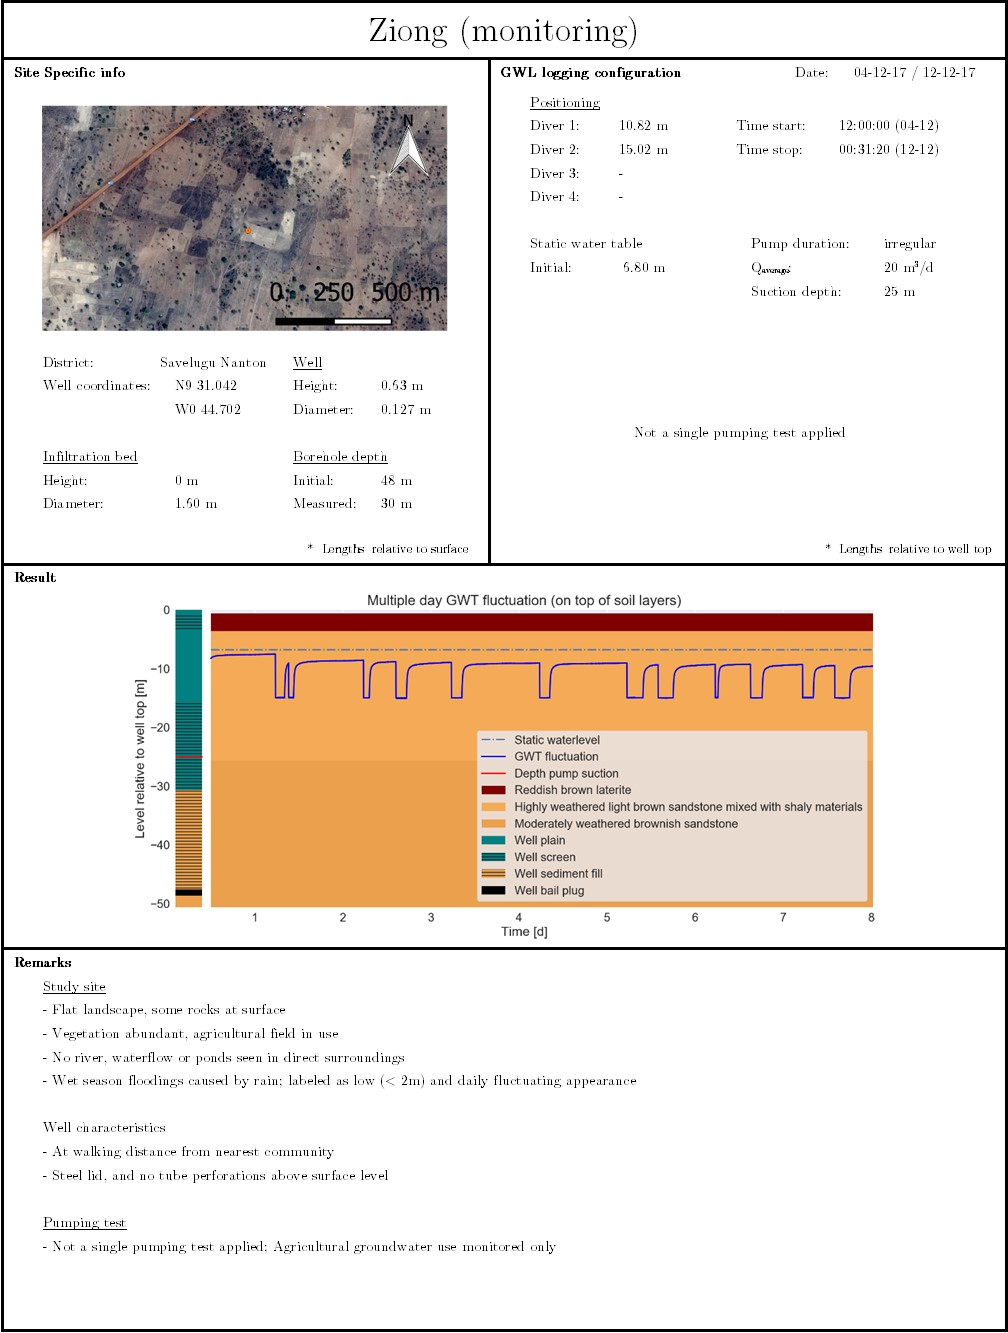
\includegraphics[width=\linewidth]{Ziong.jpg}
 \captionsetup{justification=centering}
 \caption{Fieldwork fact sheet: Ziong (location of monitoring)}
 \label{fig:Ziong}
\end{figure} 